\chapter{Background}

\section{Databases}

A database \cite{8} is an organized collection of data, which can be managed in an easy way. A database management system is a computer software application 
that interacts with the user and other applications, in order to create, access, manage and execute queries at the data stored in the database. 
Databases are used in a wide range of services, such as bank, university and communication platforms. 

\subsection{Relational databases}

A relational database is a digital database whose organization is based on the relational model of data \cite{9}. According to this model, data are organized in tables 
with rows and columns. Each table represents a relation variable, each row is an implementation of this variable and each column is an attribute of the variable. 
Tables can be associated with one-to-one, one-to-many and many-to-many relationships. More specifically, a relation is a set of table rows that have common attributes. 
Moreover, each row can be uniquely identified by a certain attribute, called primary key. When a primary key is common between two tables, then it becomes 
a foreign key for the second table. Finally, a database index is a data structure that improves the speed of data retrieval operations on a database table 
at the cost of additional writes and storage space to maintain the index data structure.

\subsection{ACID properties}

ACID (Atomicity, Consistency, Isolation, Durability) \cite{10} is a set of properties that guarantee that database transactions are processed reliably. 
In the context of databases, a single logical operation on the data is called a transaction. 

\subsubsection{Atomicity}

Atomicity requires that each transaction be "all or nothing": 
if one part of the transaction fails, the entire transaction fails, and the database state is left unchanged. An atomic system must guarantee atomicity in each 
and every situation, including power failures, errors, and crashes. To the outside world, a committed transaction appears (by its effects on the database) to be 
indivisible ("atomic"), and an aborted transaction does not happen.

\subsubsection{Consistency}

The consistency property ensures that any transaction will bring the database from one valid state to another. Any data written to the database must be valid 
according to all defined rules, including constraints, cascades, triggers, and any combination thereof. This does not guarantee correctness of the transaction 
in all ways the application programmer might have wanted (that is the responsibility of application-level code) but merely that any programming errors cannot 
result in the violation of any defined rules.

\subsubsection{Isolation}

The isolation property ensures that the concurrent execution of transactions results in a system state that would be obtained if transactions were 
executed serially. Providing isolation is the main goal of concurrency control. Depending on concurrency control method 
(i.e. if it uses strict - as opposed to relaxed - serializability), the effects of an incomplete transaction might not even be visible to another transaction.

\subsubsection{Durability}

Durability means that once a transaction has been committed, it will remain so, even in the event of power loss, crashes, or errors. In a relational database, 
for instance, once a group of SQL statements execute, the results need to be stored permanently (even if the database crashes immediately thereafter). 
To defend against power loss, transactions (or their effects) must be recorded in a non-volatile memory.

\subsection{OLTP vs OLAP}

\subsubsection{OLTP}

Online transaction processing, or OLTP, is a class of information systems that facilitate and manage transaction-oriented applications, typically for 
data entry and retrieval transaction processing. OLTP is characterized by a large number of short on-line transactions (INSERT, UPDATE, DELETE). 
OLTP must possess ACID qualities to maintain data integrity and to ensure that transactions are correctly executed. 
The main emphasis for OLTP systems is put on very fast query processing, maintaining data integrity in multi-access environments and an effectiveness 
measured by number of transactions per second. In OLTP database there is detailed and current data, and the schema used to store transactional databases is the entity model.

\subsubsection{OLAP}
Online analytical processing, or OLAP, is characterized by relatively low volume of transactions. Queries are often very complex and involve aggregations. 
For OLAP systems a response time is an effectiveness measure. OLAP applications are widely used by Data Mining techniques. 
In OLAP database there is aggregated, historical data, stored in multi-dimensional schemas.

\section{PostgreSQL}

PostgreSQL \cite{11} is an open source object-relational database management system. It runs on all major operating systems, including Linux, UNIX (AIX, BSD, HP-UX, 
SGI IRIX, Mac OS X, Solaris, Tru64), and Windows. It is fully ACID compliant, has full support for foreign keys, joins, views, triggers, and stored procedures 
(in multiple languages). It includes most SQL:2008 data types, including INTEGER, NUMERIC, BOOLEAN, CHAR, VARCHAR, DATE, INTERVAL, and TIMESTAMP. It also supports 
storage of binary large objects, including pictures, sounds, or video. Moreover, it has native programming interfaces for C/C++, Java, .Net, Perl, Python, Ruby, Tcl, ODBC. 
It supports international character sets, multibyte character encodings, Unicode, and it is locale-aware for sorting, case-sensitivity, and formatting. 
In addition, it supports unlimited database size, rows and indexes per table, 32TB table size, 1.6TB row size and 1GB field size. PostgreSQL manages 
database access permissions using the concept of roles. A role can be thought of as either a database user, or a group of database users, depending on how 
the role is set up. Roles can own database objects (for example, tables) and can assign privileges on those objects to other roles to control 
who has access to which objects. Furthermore, it is possible to grant membership in a role to another role, thus allowing the member role use of privileges 
assigned to the role it is a member of. Finally, PostgreSQL comes with several extensions that add extra capabilities in its function and usage. 

\subsection{PostGIS}

PostGIS \cite{12} is a spatial database extender for PostgreSQL object-relational database. It adds support for geographic objects allowing location queries 
to be run in SQL. It defines new data types, functions, operators and indexes especially for geographic objects. 

\subsubsection{Geography type}

The geography type provides native support for spatial features represented on geographic coordinates. A specific point on a map can be identified by it's 
geographic coordinates, stated in the form of (latitude, longitude). Geographic coordinates are spherical coordinates expressed in angular units (degrees). 
The basis for the PostGIS geographic type is a sphere. The shortest path between two points on the sphere is a great circle arc. That means that calculations 
on geographies (areas, distances, lengths, intersections, etc) must be calculated on the sphere, using more complicated mathematics. For more accurate 
measurements, the calculations must take the actual spheroidal shape of the world into account. There are several functions and operators 
that take as input or return as output a geography data type object. One very useful one, is the function ST\_DWithin. 
This function returns true if the geographies are within the specified distance of one another. Units are in meters and measurement is defaulted 
to measure around spheroid. 

\subsection{Indexes}

A database index is a data structure that improves the speed of data retrieval operations on a database table at the cost of additional writes and storage 
space to maintain the index data structure. Indexes are used to quickly locate data without having to search every row in a database table every time a database 
table is accessed. Indexes can be created using one or more columns of a database table, providing the basis for both rapid random lookups and efficient access 
of ordered records.

\subsubsection{B-tree}

PostgreSQL uses by default a B-tree index on a table column. B-tree \cite{13} is a tree data structure that keeps data sorted and allows searches, sequential access, 
insertions, and deletions in logarithmic time. The B-tree is a generalization of a binary search tree in that a node can have more than two children.
More specifically, it is a balanced tree whose nodes contain pointers to a table's records and a number of keys. The keys act as separation values which 
divide its subtrees. For example, if an internal node has 3 child nodes (or subtrees) then it must have 2 keys: a1 and a2. All values in the leftmost subtree 
will be less than a1, all values in the middle subtree will be between a1 and a2, and all values in the rightmost subtree will be greater than a2. 
Unlike self-balancing binary search trees, the B-tree is optimized for systems that read and write large blocks of data.

\subsubsection{R-tree}

R-trees \cite{14} are tree data structures used for spatial access methods, such as indexing multi-dimensional information like geographical coordinates. 
The key idea of the data structure is to group nearby objects and represent them with their minimum bounding rectangle in the next higher level of the tree; 
the "R" in R-tree is for rectangle. Since all objects lie within this bounding rectangle, a query that does not intersect the bounding rectangle also cannot 
intersect any of the contained objects. At the leaf level, each rectangle describes a single object; at higher levels the aggregation of an increasing number 
of objects. This can also be seen as an increasingly coarse approximation of the data set. 
R-tree's searching lgorithms use the bounding boxes to decide whether or not to search inside a subtree. In this way, most of the nodes in the tree are never 
read during a search. Like B-trees, this makes R-trees suitable for large data sets and databases, where nodes can be paged to memory when needed, and the whole 
tree cannot be kept in main memory. 

\subsubsection{GiST}

GiST \cite{15} stands for Generalized Search Tree. It is a balanced, tree-structured access method, that acts as a base template in which to implement arbitrary 
indexing schemes. B-trees, R-trees and many other indexing schemes can be implemented in GiST. GiST tree nodes contain a pair of values in the form of (p, prt). 
The first value, p, is used as a search key and the second value, ptr, is a pointer to the data if the node is a leaf or a pointer to another node 
if the node is intermediate. The search key p represents an attribute that becomes true for all data that can be reached through the pointer ptr. 
Also, GiST index can handle any query predicate, as long as certain functions, that influence the behavior of the search keys, are implemented. 

PostGIS can use GiST index at a table attribute. When a table column is a geography data type, then GiST will use an improved version of an R-tree index 
(R-tree-over-GiST scheme). PostgreSQL doesn't allow, at the most recent versions, the use of standard R-tree, because this type of index 
cannot handle attributes with size bigger than 8K and fail when a geography column is null. 

\section{HDFS}

The Hadoop Distributed File System (HDFS) \cite{28} is a distributed file system designed to run on commodity hardware. HDFS is highly fault-tolerant and is 
designed to be deployed on low-cost hardware. HDFS provides high throughput access to application data and is suitable for applications that have large data sets. 
HDFS is designed to reliably store very large files across machines in a large cluster. It stores each file as a sequence of blocks; all blocks in a file except 
the last block are the same size. The blocks of a file are replicated for fault tolerance.

The NameNode is the centerpiece of an HDFS file system. It keeps the directory tree of all files in the file system, and tracks where across the cluster the file data 
is kept. It does not store the data of these files itself. Client applications talk to the NameNode whenever they wish to locate a file, or when they want to 
add/copy/move/delete a file. The NameNode responds the successful requests by returning a list of relevant DataNode servers where the data lives. A Datanode 
stores data in the HDFS. Client applications can talk directly to a DataNode, once the NameNode has provided the location of the data. 
The DataNodes also perform block creation, deletion, and replication upon instruction from the NameNode. 


\section{HBase}

HBase is an open source, non-relational (NoSQL), distributed database modeled after Google's BigTable \cite{24}. It is developed as part of Apache Software Foundation's Apache 
Hadoop project and runs on top of HDFS.  

\subsection{Data model}

HBase works best for sparse data sets, which are common in many Big Data use cases. Unlike relational database systems, HBase does not support a 
structured query language like SQL; in fact, HBase isn’t a relational data store at all. HBase  is a column-oriented database and follows a 
key/value data storage model. The main characteristics if the data model are the following: 

\begin{itemize}
 \item Table: HBase organizes data into tables as most database systems.
 \item Row: Within a table, data are stored according to its row. Rows are uniquely identified by a key. Row keys are treated as byte arrays, thus they do not 
 have a specific data type.
 \item Column Family: Column families group data within a row, impacting their physical arrangement. They are stored together on disk, which is why 
 HBase is referred to as a column-oriented data store. Column families must be defined up front, during table creation. 
 \item Column Qualifier: Data within a column family are addressed via its column qualifier, or simply, column. Column qualifiers need not be consistent 
 between rows. Like row keys, column qualifiers do not have a data type and are always treated as a byte array.
 \item Cell: A combination of row key, column family, and column qualifier uniquely identifies a cell. The data stored in a cell are 
 referred to as that cell’s value. Values also do not have a data type and are always treated as a byte array.
 \item Timestamp: Values within a cell are versioned. Versions are identified by their version number, which by default is the timestamp of when the cell was written. 
If a timestamp is not specified during a write, the current timestamp is used. If the timestamp is not specified for a read, the latest one is returned. The number 
of cell value versions retained by HBase is configured for each column family. The default number of cell versions is three.
\end{itemize}

For example, a table in HBase can be the following:

\begin{figure}[H]
  \centering
  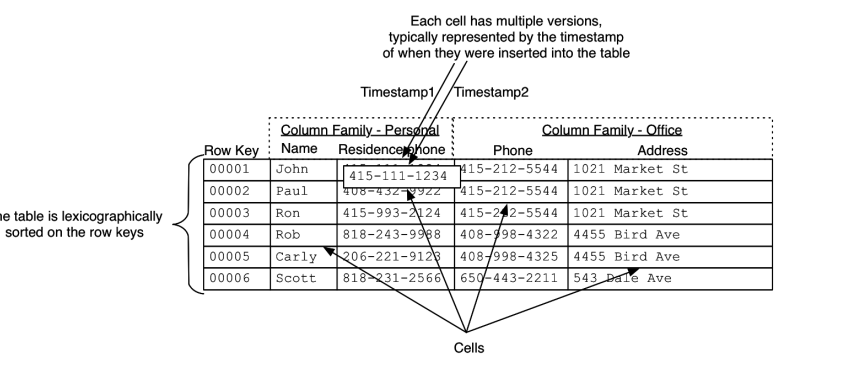
\includegraphics[width=0.9\textwidth]{figures/hbase.png}
  \caption{A table in HBase consisting of two column families}
\end{figure}

\subsection{Architecture components}

HBase has the following three major architecture components:

\begin{itemize}
 \item Region server: Regions are parts of HBase tables, splitted accross the region servers of the distributed system and managed by a region server. 
 Region server communicates with the client and handles data-related operations. Also, it handles read and write requests for all regions under it and decides 
 the size of the regions.
 \item Master server: Master server assigns regions to the region servers and handles the load balancing of the regions across region servers. Moreover, it is 
 responsible for schema changes and other metadata operations such as creation of tables and column families. 
 \item Zookeeper: Zookeeper server is responsible to handle and synchronize the communication between the master and region servers, providing 
 fault tolerance. More specifically, ZooKeeper is a centralized service for maintaining configuration information, naming, providing distributed 
 synchronization, and providing group services.
\end{itemize}

\subsection{Coprocessors}

HBase coprocessors \cite{30} enable distributed computation directly within the HBase server processes on the server's local data.
The idea of HBase Coprocessors was inspired by Google’s BigTable coprocessors. Coprocessors can be loaded globally on all tables and regions hosted 
by the region server, these are known as system coprocessors; or the administrator can specify which coprocessors should be loaded on all regions for a table on 
a per-table basis, these are known as table coprocessors. There are two categories of HBase coprocessors, the observer and the 
endpoint coprocessors. The idea behind observers is that we can insert user code by overriding upcall methods provided by the coprocessor framework. 
The callback functions are executed from core HBase code when certain events occur. 
Endpoints, on the other hand, are more powerful, resembling stored procedures. One can invoke an endpoint at any time from the client. The endpoint implementation 
will then be executed remotely at the target region or regions, and results from those executions will be returned to the client. 
In essence, coprocessors implement the idea of "move computation near the data", a method that google heavily utilizes to increase performance: it is much cheaper 
to transfer a small piece of code to be executed in parallel in various servers instead of moving data where the code is installed.

The Endpoint is an interface for dynamic RPC extension. The endpoint implementation is installed on the server side and can then be invoked with an HBase RPC. 
The client library provides convenience methods for invoking such dynamic interfaces. The application code client side performs a batch call. 
This initiates parallel RPC invocations of the registered dynamic protocol on every target table region. The results of those invocations are returned 
as they become available. The client library manages this parallel communication on behalf of the application, messy details such as dealing with retries 
and errors, until all results are returned (or in the event of an unrecoverable error). Then the client library rolls up the responses into a Map and hands 
it over to the application. If an unrecoverable error occurs, then an exception will be thrown for the application code to catch and take action.


\section{Google Maps Directions API}

The Google Directions API \cite{16} is a service that calculates directions between locations using an HTTP request. A Directions API request takes the following form:
\begin{center}
  http://maps.googleapis.com/maps/api/directions/output?parameters
\end{center}

where output determines the type of file that will contain the answer to the HTTP request. The type of the output file can be either json of xml. 
The field parameters 
defines the parameters and their values that will come along with the HTTP request. Certain parameters are required while others are optional. As is standard 
in URLs, all parameters are separated using the ampersand (\&) character. Required parameters are the origin and destination locations between which we 
request directions through the Directions API. These locations can be in the form of textual geographical coordinates as a value pair of latitude and 
longitude. Location can also be inserted as the address of the specific point. In this case, Directions service will geocode the string and convert it to 
a latitude/longitude coordinate in order to calculate directions. Other optional parameters, that can be defined, are the mode of transportation, 
which can be driving, walking, bicycling, or transit. For example, a complete HTTP request to the Directions API can be the following:

\begin{center}
 http://maps.googleapis.com/maps/api/directions/json?origin=37.976159, 23.776274\&destination=37.978180, 23.768957\&mode=walking
\end{center}

\subsection{JSON response file}

JSON (JavaScript Object Notation) file format, is an open standard format that uses human-readable text to transmit data objects consisting of attribute–value pairs. 
Directions responses in json type format contain the following fields: 

\subsubsection{Status}

The status field within the Directions response object contains the status of the request, and may contain debugging information to help you track down why 
the Directions service failed. The status field may contain the following values:

\begin{itemize}
 \item OK, the response contains a valid result. 
 \item NOT\_FOUND, at least one of the locations specified in the request's origin, destination, or waypoints could not be geocoded.
 \item ZERO\_RESULTS, no route could be found between the origin and destination.
 \item INVALID\_REQUEST, the provided request was invalid. Common causes of this status include an invalid parameter or parameter value.
 \item REQUEST\_DENIED, the service denied use of the directions service by your application. 
 \item UNKNOWN\_ERROR, a directions request could not be processed due to a server error. 
 \item OVER\_QUERY\_LIMIT, the service has received too many requests from your application within the allowed time period. 
 More specifically, users of the free Directions API are able to perform at most 2 HTTP request per second and 2500 HTTP requests per day to the API.

\end{itemize}

For example:

\begin{lstlisting}[basicstyle=\footnotesize\ttfamily, breaklines=true]
 "status" : "OK"
\end{lstlisting}

\subsubsection{Routes}

Routes field is a JSON array, whose elements represent a different route between the origin and destination locations. Each route can contain the following 
fields:

\begin{itemize}
 \item summary: a short textual description for the route, suitable for naming and disambiguating the route from alternatives.
 \item legs[]: an array which contains information about a leg (i.e. a part) of the route, between two locations within the given route. If there are no 
 waypoints defined, the array will include one element, which will be the total route. 
 \item waypoint\_order: an array indicating the order of any waypoints in the calculated route. 
 \item overview\_polyline: a single points object that holds an encoded polyline representation of the route. This polyline is an approximate 
 (smoothed) path of the resulting directions.
 \item bounds: the viewport bounding box of the overview\_polyline.
 \item copyrights: the copyrights text to be displayed for this route. 
 \item warnings[]: an array of warnings to be displayed when showing these directions.
\end{itemize}

For example:

\begin{lstlisting}[basicstyle=\footnotesize\ttfamily, breaklines=true]
	"bounds" : {
            "northeast" : {
               "lat" : 37.97818609999999,
               "lng" : 23.7762659
            },
            "southwest" : {
               "lat" : 37.9761428,
               "lng" : 23.7689148
            }
         },
         "copyrights" : "Map data ©2015 Google",
         "legs" : [
	    ... ]
	 "overview_polyline" : {
            "points" : "{exfFuxbpCg@fCkBpK}B~MkB|KIf@QG"
         },
         "summary" : "Λεωφ. Στρατάρχου Αλεξάνδρου Παπάγου",
         "warnings" : [
            "Walking directions are in beta.    Use caution – This route may be missing sidewalks or pedestrian paths."
         ],
         "waypoint_order" : []   
\end{lstlisting}

\subsubsection{legs[]}

Each element in the legs array specifies a single leg of the journey from the origin to the destination in the calculated route. For routes that contain 
no waypoints, the route will consist of a single "leg," but for routes that define one or more waypoints, the route will consist of one or more legs, 
corresponding to the specific legs of the journey.

Each leg within the legs field(s) may contain the following fields:

\begin{itemize}
 \item steps[]: an array of steps denoting information about each separate step of the leg of the journey.
 \item distance: the total distance covered by this leg, where value field contains the distance in meters and text field contains a human-readable representation of 
 the distance, displayed in units as used at the origin
 \item duration: the total duration of this leg, where value field contains the duration in seconds and text field contains a human-readable representation of the duration.
 \item start\_location: contains the latitude/longitude coordinates of the origin of this leg. Because the Directions API calculates directions between locations 
 by using the nearest transportation option (usually a road) at the start and end points, start\_location may be different than the provided origin of this leg 
 if, for example, a road is not near the origin.
 \item start\_address: contains the human-readable address (typically a street address) reflecting the start\_location of this leg.
 \item end\_location: contains the latitude/longitude coordinates of the given destination of this leg. Because the Directions API calculates directions 
 between locations by using the nearest transportation option (usually a road) at the start and end points, end\_location may be different than the provided 
 destination of this leg if, for example, a road is not near the destination.
 \item end\_address: contains the human-readable address (typically a street address) reflecting the end\_location of this leg.
\end{itemize}

For example:

\begin{lstlisting}[basicstyle=\footnotesize\ttfamily, breaklines=true]
	      "distance" : {
                  "text" : "0.7 km",
                  "value" : 690
               },
               "duration" : {
                  "text" : "7 mins",
                  "value" : 434
               },
               "end_address" : "Iasona Maratou 509, Zografou 157 73, Greece",
               "end_location" : {
                  "lat" : 37.97818609999999,
                  "lng" : 23.7689477
               },
               "start_address" : "Papagou 147, Zografou 157 73, Greece",
               "start_location" : {
                  "lat" : 37.9761428,
                  "lng" : 23.7762659
               },
               "steps" : [
		    .... ]
\end{lstlisting}

\subsubsection{steps[]}

Each element in the steps array defines a single step of the calculated directions. A step is the most 
atomic unit of a direction's route, containing a single step describing a specific, single instruction on the journey. 
The step not only describes the instruction but also contains distance and duration information relating to how this step relates to the following step. 
Each step within the steps field(s) may contain the following fields:

\begin{itemize}
 \item html\_instructions: formatted instructions for this step, presented as an HTML text string. 
 \item distance: the distance covered by this step until the next step.
 \item duration: the time required to perform the step, until the next step.
 \item start\_location: the geographical coordinated of the location of the starting point of this step.
 \item end\_location: the geographical coordinated of the location of the last point of this step.
 \item polyline: a single points object that holds an encoded polyline representation of the step. This polyline is an approximate (smoothed) path of the step.
 \item travel\_mode: the mode of transportation, as it is defined in the mode parameter of the HTTP request.
\end{itemize}

For example:

\begin{lstlisting}[basicstyle=\footnotesize\ttfamily, breaklines=true]
	"distance" : {
           "text" : "0.7 km",
           "value" : 680
        },
        "duration" : {
           "text" : "7 mins",
           "value" : 427
        },
        "end_location" : {
           "lat" : 37.9781038,
           "lng" : 23.7689148
        },
        "html_instructions" : "Head \u003cb\u003ewest\u003c/b\u003e on \u003cb\u003eΛεωφ. Στρατάρχου Αλεξάνδρου Παπάγου\u003c/b\u003e toward \u003cb\u003eΓρ. Κουσίδη\u003c/b\u003e",
        "polyline" : {
           "points" : "{exfFuxbpCQv@ETCLKj@CPYxAi@|Cc@fCm@lDg@pCCNc@nC_AnFCHYhBMx@If@"
        },
        "start_location" : {
           "lat" : 37.9761428,
           "lng" : 23.7762659
        },
        "travel_mode" : "WALKING"
\end{lstlisting}


\subsection{Encoded Polyline Algorithm Format}

The JSON response file contains an encoded polyline as a representation of the route. This representation is the result of encoding 
the geographical coordinates of the intermediate points of the route. Google Maps API follows a specific encoding algorithm \cite{17} of the latitude and longitude 
of any point. The steps for encoding such a signed value indicating the latitude or longitude are specified below:

\begin{enumerate}
 \item Multiply the initial signed value by 1e5, rounding the result.
 \item Convert the result to it's binary equivalent value, using it's two complement. 
 \item Left-shift the binary value one bit.
 \item If the original decimal value is negative, invert this encoding.
 \item Break the binary value out into 5-bit chunks (starting from the right hand side.
 \item Place the 5-bit chunks into reverse order.
 \item OR each value with 0x20 if another bit chunk follows.
 \item Convert each value to decimal.
 \item Add 63 to each value.
 \item Convert each value to its ASCII equivalent.
\end{enumerate}

Following these steps in reverse we can decode an encoded polyline into the appropriate list of geographical coordinates 
and extract the GPS traces that define the route. 

\section{Google Maps Static Maps API}

The Google Static Map service \cite{18} creates a map based on URL parameters sent through a standard HTTP request and returns the map as an image 
that can be displayed on a web page, or accessed through a URL. A simple HTTP request to the Google Static Maps API takes the following form:

\begin{center}
 https://maps.googleapis.com/maps/api/staticmap?parameters
\end{center}

The Static Maps API defines map images using the following URL parameters:

\subsubsection{Location Parameters}

\begin{itemize}
 \item center: defines the center of the map, equidistant from all edges of the map. This parameter takes a location as either a comma-separated {latitude,longitude} 
 pair or a string address identifying a unique location on the face of the earth.
 \item zoom: defines the zoom level of the map, which determines the magnification level of the map. 
\end{itemize}

\subsubsection{Map Parameters}

\begin{itemize}
 \item size: the rectangular dimensions of the map image. This parameter takes a string of the form \{horizontal\_value\}x\{vertical\_value\}. 
 \item scale: affects the number of pixels that are returned. scale=2 returns twice as many pixels as scale=1 while retaining the same coverage area and level of detail.
 \item format: the format of the resulting image. Possible formats include PNG, GIF and JPEG types.
 \item maptype: the type of map to construct. There are several possible maptype values, including roadmap, satellite, hybrid, and terrain. 
 \item language: the language to use for display of labels on map tiles.
\end{itemize}

\subsubsection{Feature Parameters}

\begin{itemize}
 \item markers: one or more markers to attach to the image at specified locations. This parameter takes a single marker definition with parameters separated 
 by the pipe character (|). 
 \item path: a single path of two or more connected points to overlay on the image at specified locations. This parameter takes a string of point definitions 
 separated by the pipe character (|). In addition, the encoded polyline representation can be used instead of multiple points, as long as the prefix enc: 
 is used in the value of the parameter path.
 \item visible: one or more locations that should remain visible on the map, though no markers or other indicators will be displayed. 
\end{itemize}

For example, a HTTP request at Google Static Maps API can be the following:

\begin{center}
 https://maps.googleapis.com/maps/api/staticmap?\&size=1000x1000\&markers=label:A|17.7466,-64.703\&markers=label:C|17.7453,-64.7019\&path=color:blue|enc:gcikBvh|iKFJ??nAaAFGjA\}@rAiAJK
\end{center}

\section{Mathematical Background}

\subsection{Random Variables}

A random variable X is a measurable function from the set of possible outcomes Ω, Χ: Ω\(\rightarrow\)A or Χ: Ω\(\rightarrow\)R, where A is a 
subset of the set of real numbers. If A is a set of discrete values, such as the set of integer numbers, then the random variable is discrete. 
If A is a set of infinite possible values, then the random variable is continuous. In general, a random variable is a variable whose value is 
subject to variations due to chance. A random variable can take on a set of possible different values (similarly to other mathematical variables), 
each with an associated probability if the variable is discrete, or with a probability density function if the variable is continuous. 
The function of the random variable is called probability distribution.

\subsection{Uniform Distribution}

The discrete uniform distribution is a symmetric probability distribution whereby a finite number of values are equally likely to be observed; 
every one of n values has equal probability 1/n. 

\begin{figure}[H]
  \centering
  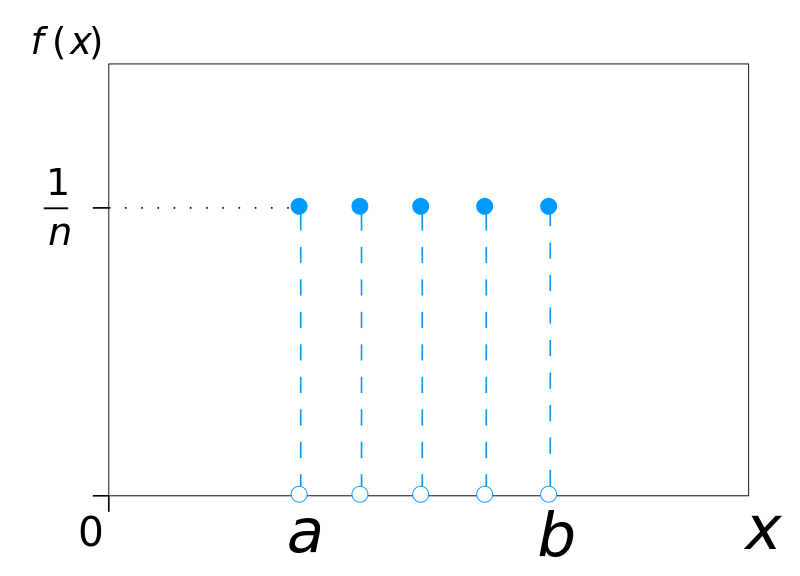
\includegraphics[width=0.5\textwidth]{figures/uniform_1.png}
  \caption{Discrete uniform probability mass function}
\end{figure}

\begin{figure}[H]
  \centering
  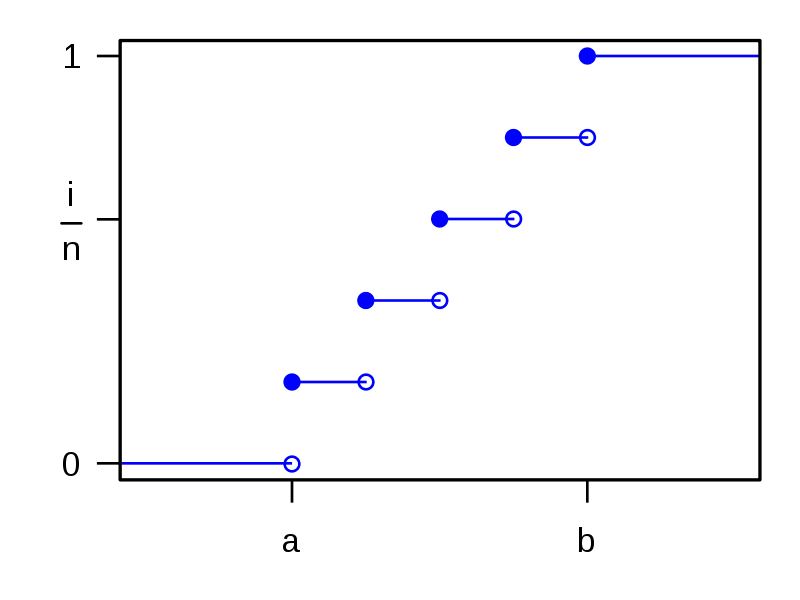
\includegraphics[width=0.5\textwidth]{figures/uniform_2.png}
  \caption{Discrete uniform cumulative distribution function}
\end{figure}

\subsection{Normal Distribution}

Normal distribution, known also as Gauss distribution, refers to continuous random variables. 
The normal distribution is remarkably useful because of the central limit theorem. In its most general form, it states that averages of random variables 
drawn from independent distributions are normally distributed. The probability density of the normal distribution is:

\[P(x) = \frac{1}{{\sigma \sqrt {2\pi } }}e^{{{ - \left( {x - \mu } \right)^2 } \mathord{\left/ {\vphantom {{ - \left( {x - \mu } \right)^2 } {2\sigma ^2 }}} \right. \kern-\nulldelimiterspace} {2\sigma ^2 }}}\]

where \(\mu\) is the mean of the distribution and \(\sigma\) is the standard deviation of the distribution.

\begin{figure}[H]
  \centering
  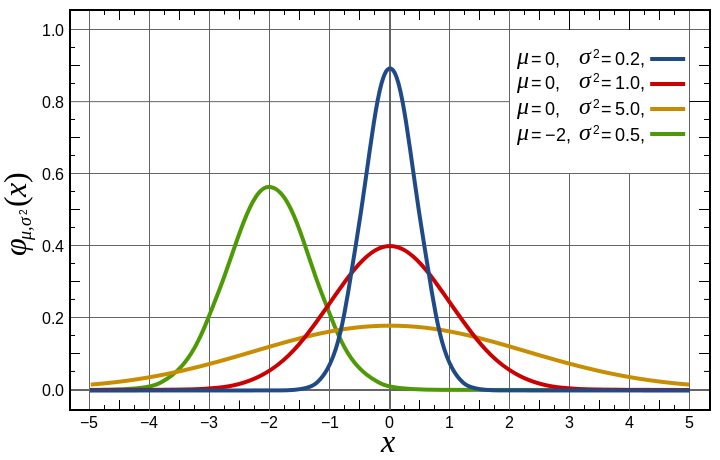
\includegraphics[width=0.5\textwidth]{figures/gauss_1.png}
  \caption{Probability density function}
\end{figure}

\begin{figure}[H]
  \centering
  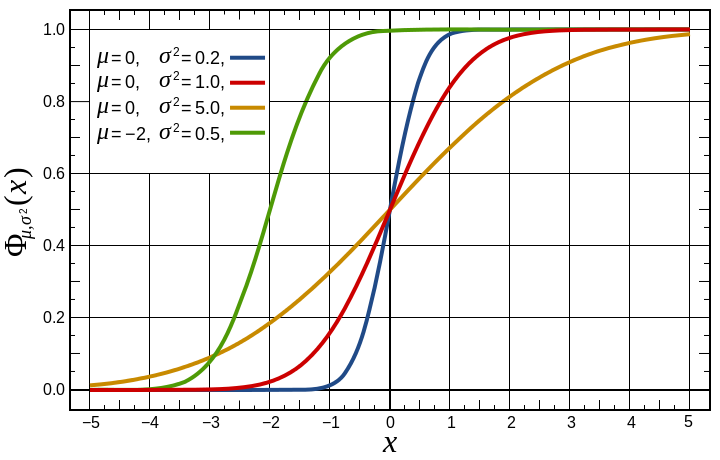
\includegraphics[width=0.5\textwidth]{figures/gauss_2.png}
  \caption{Cumulative distribution function}
\end{figure}

According to an empirical rule, about 68\% of values drawn from a normal distribution are within one standard deviation \(\sigma\) away from the mean; 
about 95\% of the values lie within two standard deviations; and about 99.7\% are within three standard deviations. This fact is known as the 68-95-99.7 
rule, or the 3-sigma rule.

\begin{figure}[H]
  \centering
  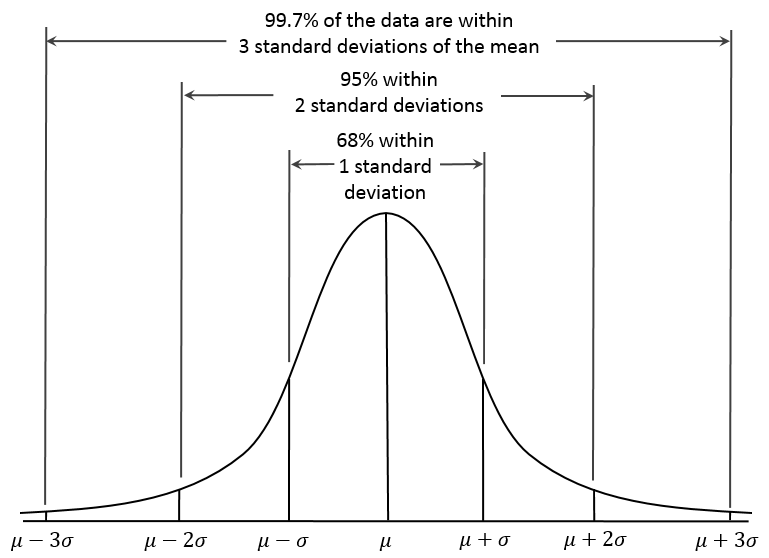
\includegraphics[width=0.6\textwidth]{figures/Empirical_Rule.PNG}
  \caption{3-sigma empirical rule for the normal distribution}
\end{figure}

\subsection{Bernoulli Distribution}

The Bernoulli distribution is the probability distribution of a random variable which takes value 1 with success probability p and value 0 with failure 
probability q=1-p. It can be used, for example, to represent the toss of a (not necessarily fair) coin, where "1" is defined to mean "heads" and "0" is 
defined to mean "tails" (or vice versa).

If X is a random variable with this distribution, we have:

\[P(X=1) = p\]
\[P(X=0) = 1-p\]

The experiment is called fair if p=0.5 and can represent the toss of a fair coin. 
















